\chapter{High fidelity prototype}


\section{Prototype}
The last iteration of the prototype is the High fidelity prototype. This prototype is as close as it gets to the final product. Therefore the focus of this iteration was to make the prototype look and feel as nice as possible.\\
This prototype is made in a real programming language and in the style which matches the windows store app's.\\
These app's are commonly very simple and very easy to use. This helps achieving our most important usability and user experience goals.\\
Since the app is simple it doesn't over complicate the task at hand by fancy graphics. This makes the app helpful for the caregivers and hopefully also satisfying to use too. With this in mind it achieves most usability goals - effectiveness, efficiency, learnable and memorable. These goals are all achieved when the app is simple and manageable.\\
As it shows with the comparison below, the prototype is simpler and more beautiful than the mid fidelity prototype.\\
\begin{figure}[H]
\centering
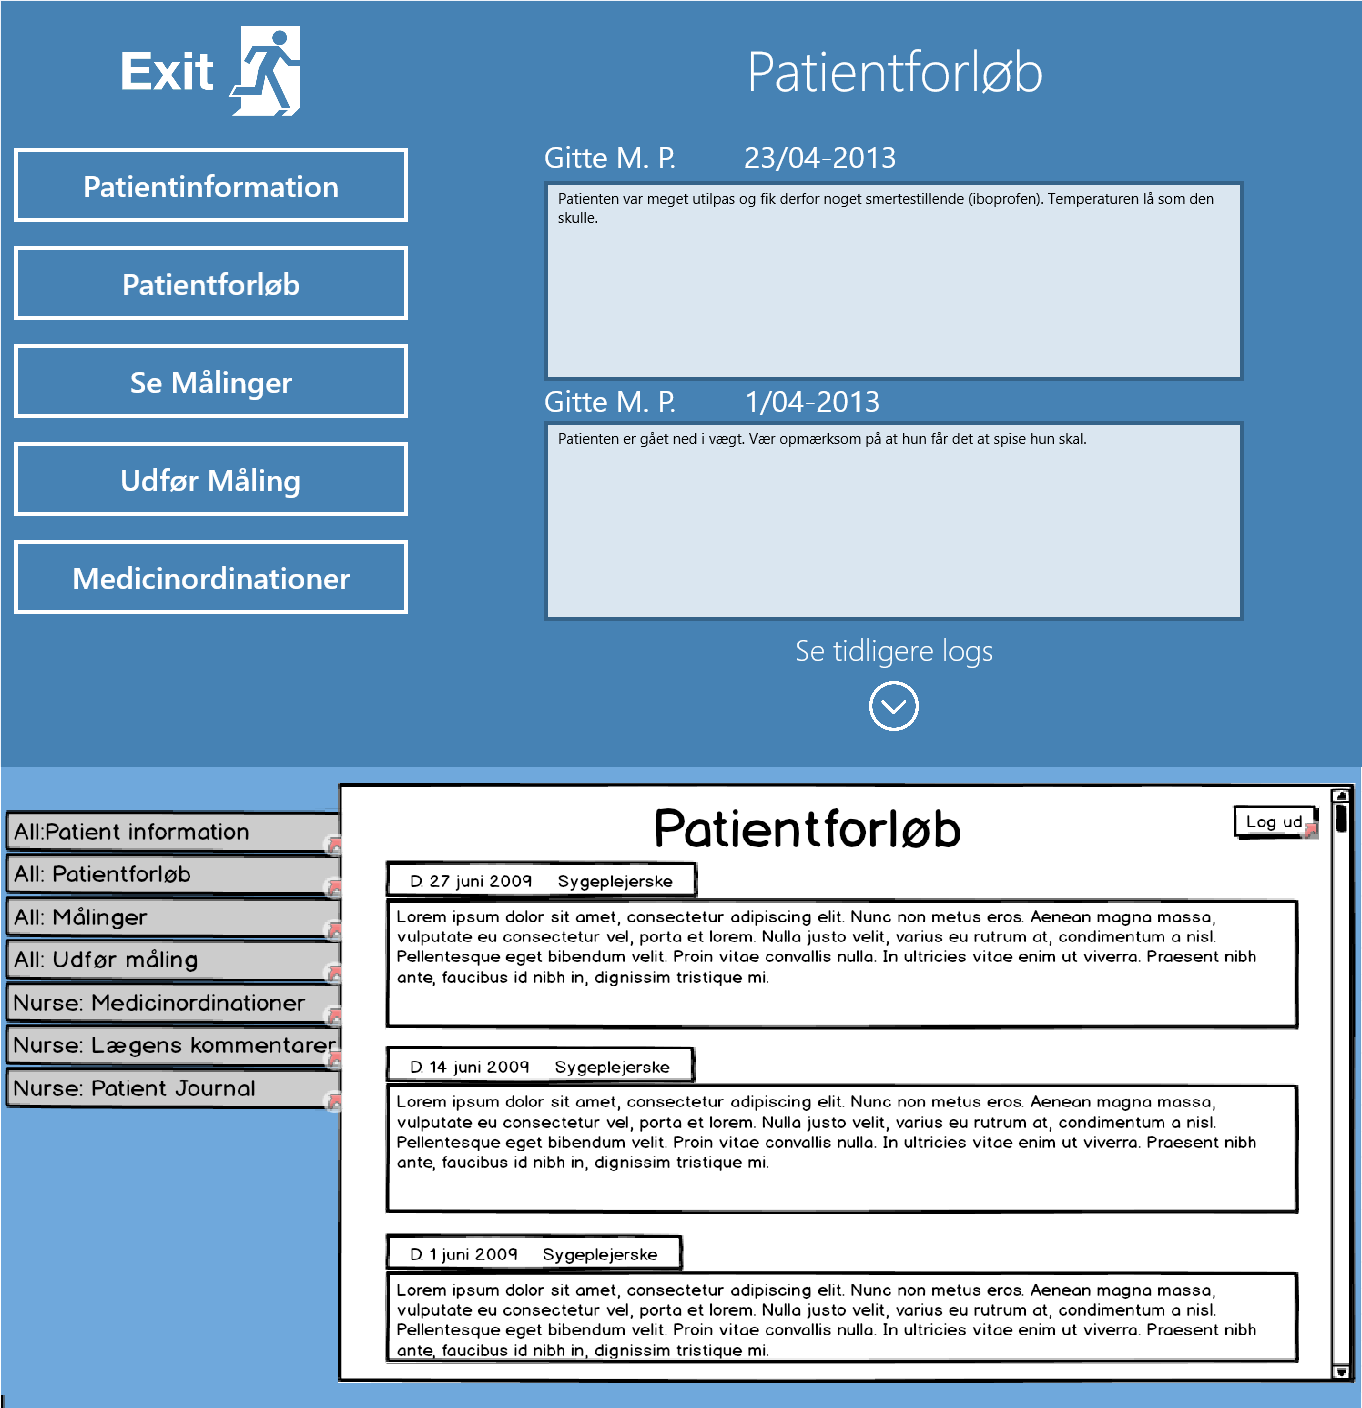
\includegraphics[width=.65\textwidth]{billeder/midhigh_compare.png}
\caption{Mid and High fidelity comparison}
\end{figure}
The overall thought behind the prototype is simple and clear buttons with one or two words very precisely describing what it leads to. The philosophy behind this is from the book "Don't make me think"(Steve Krug, 2006). Even though this book is for web development, the points and thought behind are very relevant when developing anything with a graphical user interface.\\
The prototype also doesn't have a whole lot of pages inside pages, the prototype structure is very flat. This would lead to confusion and raise questions from the user like "Where am i now?" or "How do i get to...?". Below is shown a system overview. It shows how few subpages there are. Worth mentioning is that even though all arrows in the "patient login" only goes from "Patient information" and to the other pages, the buttons still stay in the left side and you can with one click get to all the other pages.\\
\begin{figure}[H]
\centering
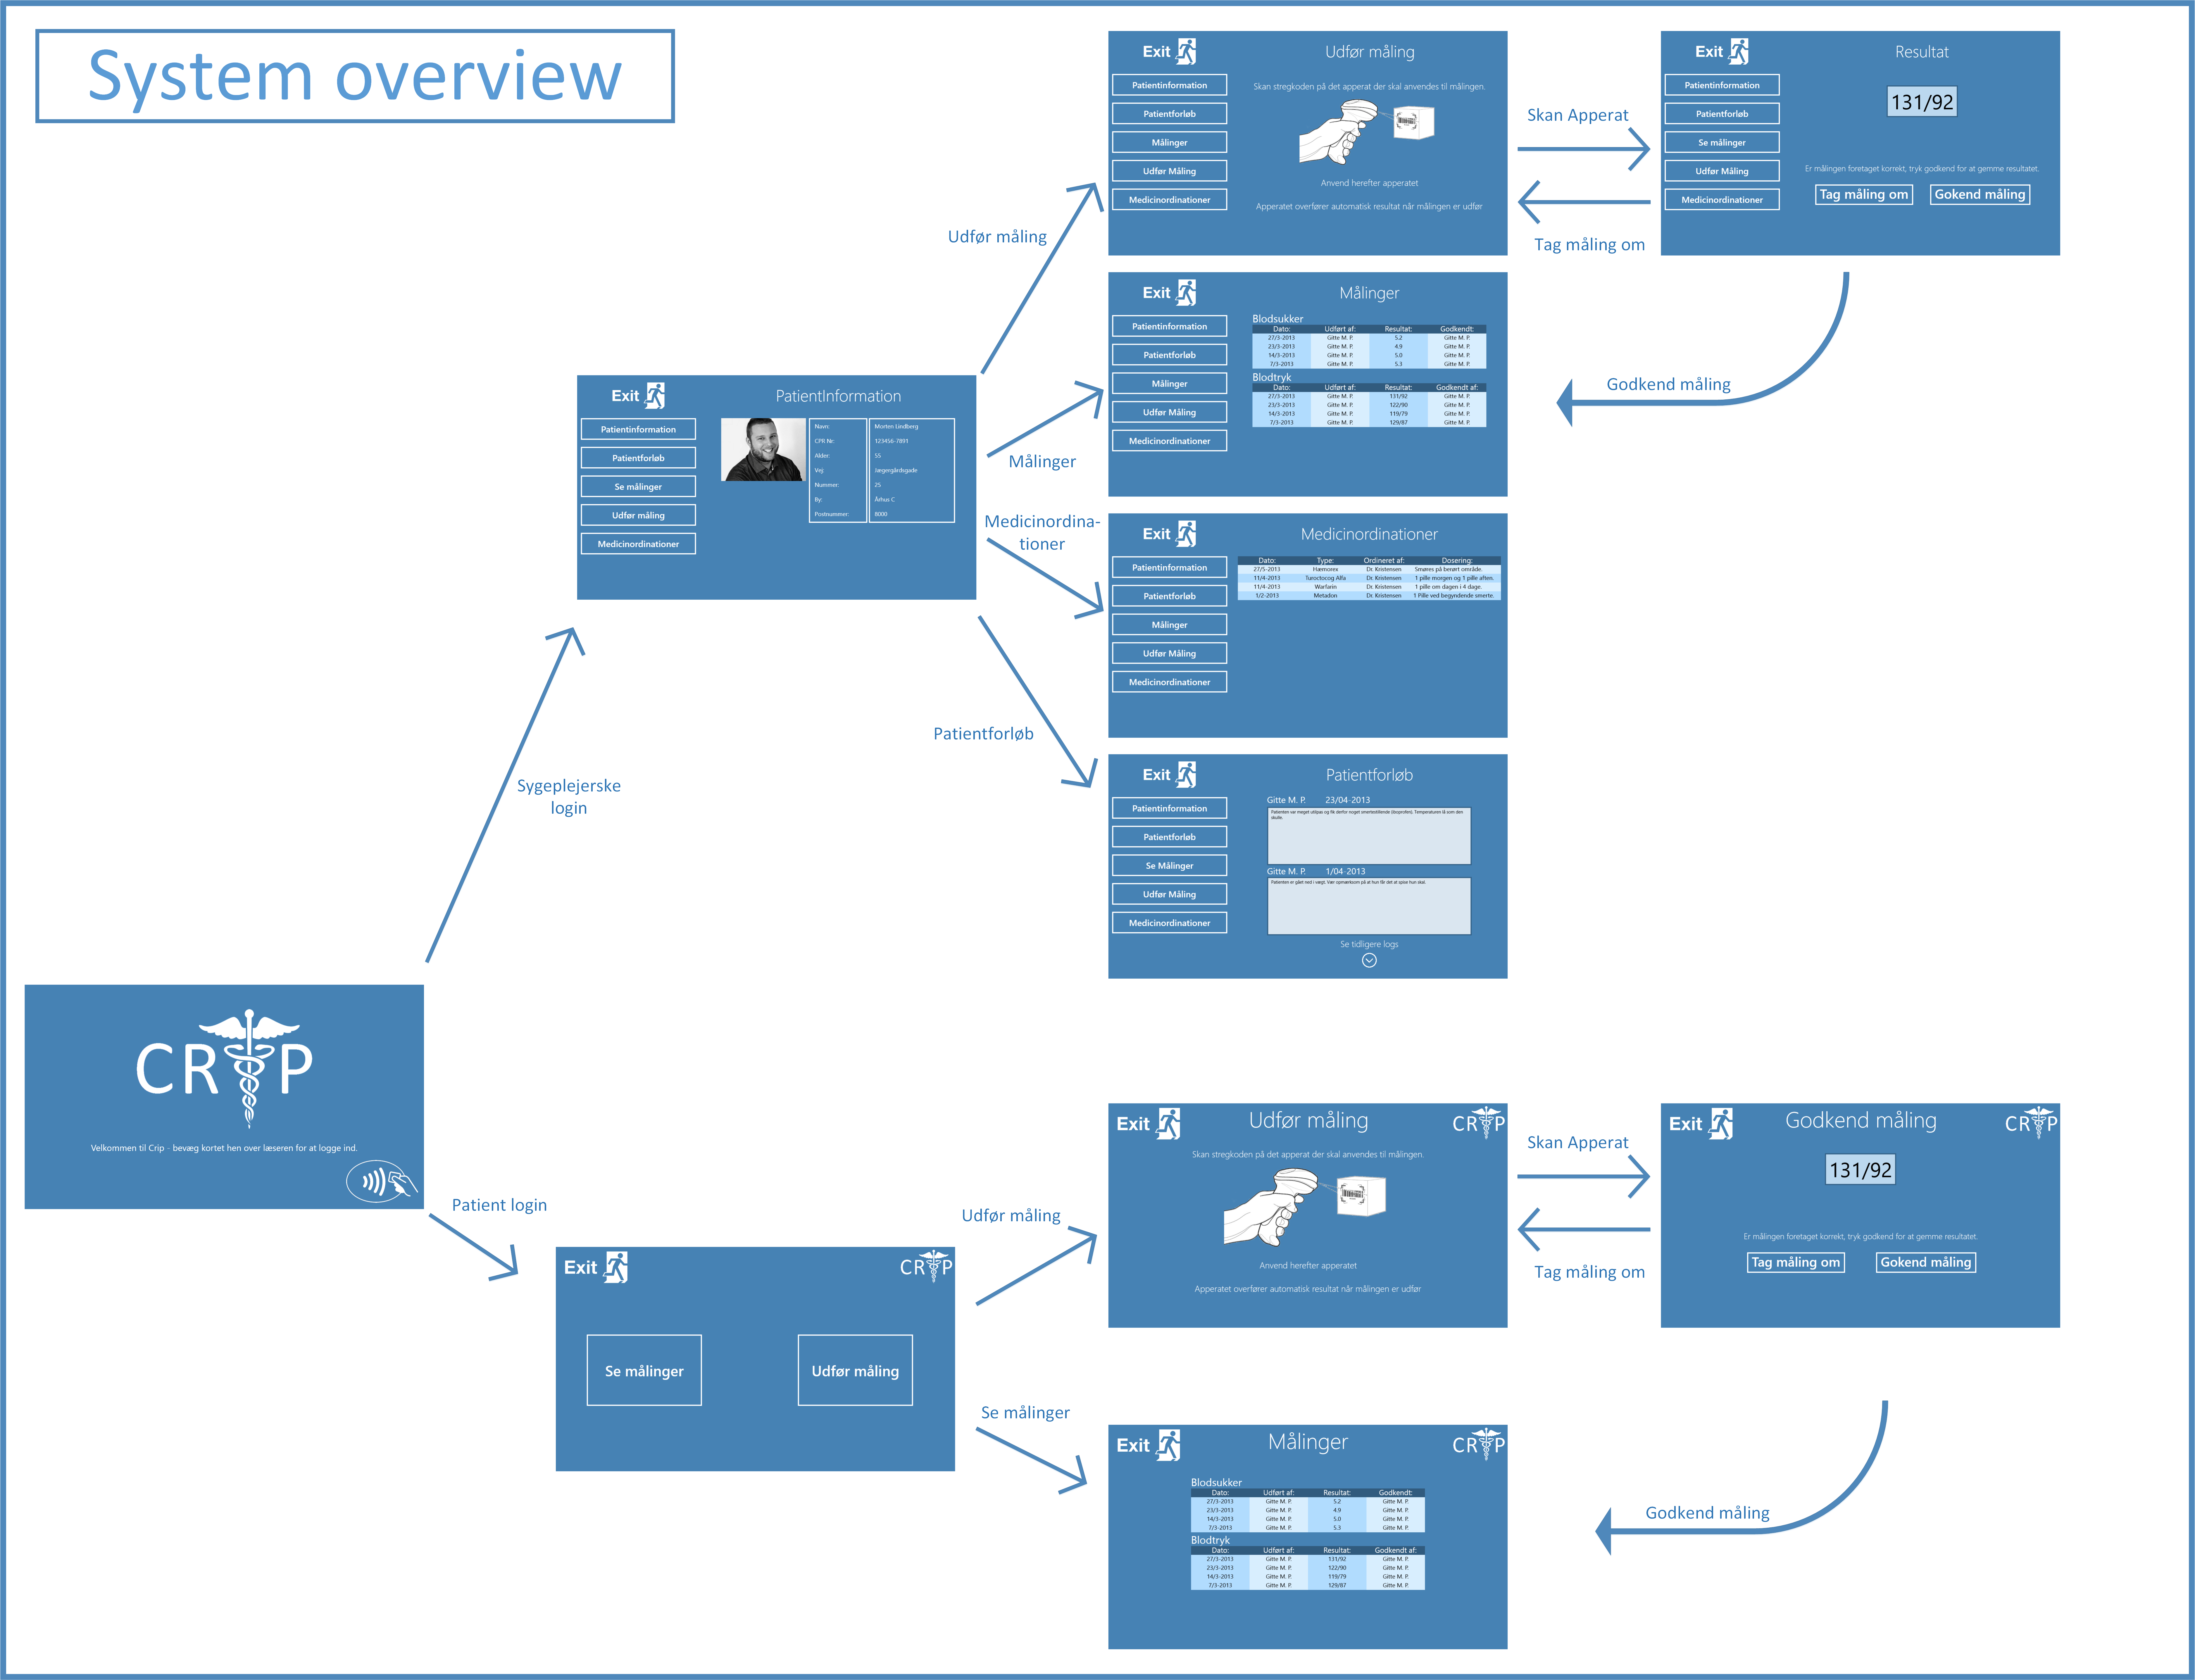
\includegraphics[width=1\textwidth]{billeder/system_hifi.png}
\caption{System overview}
\end{figure}
For a user (nurse or patient) they simply have to swipe their card (with RFID tag) over the reader next to the screen and they are presented with their "Main Page". In the nurse perspective it is the "Patient information" and in the patient perspective it is the "Se målinger/Udfør målinger" page.\\
The last thing changed in the hifi prototype is the user levels. Since the system should be able to handle patients making measurements themselves we didn't want to present them with trivial/unimportant information. Therefore the patient will be presented with a much simpler interface when signing in with the RFID card. Below is shown the patient main page.\\
\begin{figure}[H]
\centering
\includegraphics[width=.7\textwidth]{billeder/usermainpage_hifi.png}
\caption{Patient main page.}
\end{figure}
The design with the two large buttons/tiles was a result of a discussion with the peer review group.\\
\section{Peer review}
Hest

\subsection{Results of hi-fi peer review}
Hest